Java is a general-purpose computer programming language that is concurrent, class-based, object-oriented, and specifically designed to have as few implementation dependencies as possible. It is intended to let application developers "write once, run anywhere" (WORA),[15] meaning that compiled Java code can run on all platforms that support Java without the need for recompilation. Java applications are typically compiled to byte code that can run on any Java virtual machine (JVM) regardless of computer architecture. As of 2016, Java is one of the most popular programming languages in use, particularly for client-server web applications, with a reported 9 million developers. Java was originally developed by James Gosling at Sun Microsystems (which has since been acquired by Oracle Corporation) and released in 1995 as a core component of Sun Microsystems' Java platform. The language derives much of its syntax from C and C++, but it has fewer low-level facilities than either of them.

\begin{figure}[ht]
\centering
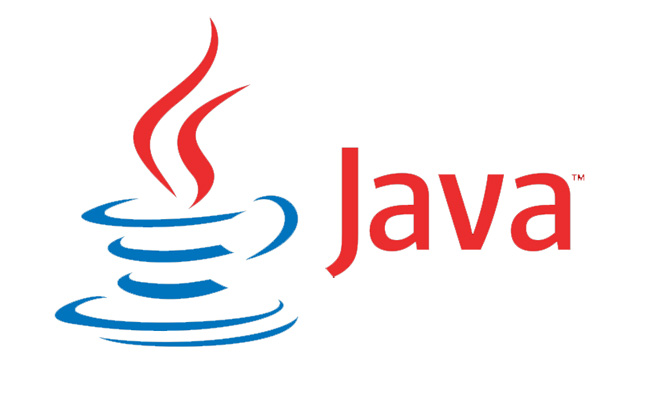
\includegraphics[scale=0.5]{images/java.png}
\caption{Java Logo}
\end{figure}


The original and reference implementation Java compilers, virtual machines, and class libraries were originally released by Sun under proprietary licenses. As of May 2007, in compliance with the specifications of the Java Community Process, Sun relicensed most of its Java technologies under the GNU General Public License. Others have also developed alternative implementations of these Sun technologies, such as the GNU Compiler for Java (byte code compiler), GNU Class path (standard libraries), and IcedTea-Web (browser plug-in for applets).
The latest version is Java 8 which is the only version currently supported for free by Oracle, although earlier versions are supported both by Oracle and other companies on a commercial basis.

\section{Java Platform}
One design goal of Java is portability, which means that programs written for the Java platform must run similarly on any combination of hardware and operating system with adequate runtime support. This is achieved by compiling the Java language code to an intermediate representation called Java byte code, instead of directly to architecture-specific machine code. Java byte code instructions are analogous to machine code, but they are intended to be executed by a virtual machine (VM) written specifically for the host hardware. End users commonly use a Java Runtime Environment (JRE) installed on their own machine for standalone Java applications, or in a web browser for Java applets.
Standard libraries provide a generic way to access host-specific features such as graphics, threading, and networking.
The use of universal bytecode makes porting simple. However, the overhead of interpreting bytecode into machine instructions made interpreted programs almost always run more slowly than native executables. Just-in-time (JIT) compilers that compile byte codes to machine code during runtime were introduced from an early stage. Java itself is platform-independent and is adapted to the particular platform it is to run on by a Java virtual machine for it, which translates the Java byte code into the platform's machine language.

\section{Automatic Memory Management}
Java uses an automatic garbage collector to manage memory in the object lifecycle. The programmer determines when objects are created, and the Java runtime is responsible for recovering the memory once objects are no longer in use. Once no references to an object remain, the unreachable memory becomes eligible to be freed automatically by the garbage collector. Something similar to a memory leak may still occur if a programmer's code holds a reference to an object that is no longer needed, typically when objects that are no longer needed are stored in containers that are still in use. If methods for a nonexistent object are called, a "null pointer exception" is thrown. One of the ideas behind Java's automatic memory management model is that programmers can be spared the burden of having to perform manual memory management. In some languages, memory for the creation of objects is implicitly allocated on the stack or explicitly allocated and deallocated from the heap. In the latter case, the responsibility of managing memory resides with the programmer.
